
\subsection{Teil III. Feinjustierung und Konvergenz in Richtung Optimum}
\label{subsec:Fine_Tuning_and_Convergence_Towards_Optimum}

Mit fortschreitendem Training begann der Kritiker jedoch, die Lage korrekter einzuschätzen, und seine Bewertungen wurden zunehmend präziser. In der dritten Phase konnte beobachtet werden, wie der Akteur endlich begann, die angemessenen Anpassungen vorzunehmen, was zu einer allmählichen Verbesserung und Annäherung an die optimale Lösung führte. Die Richtung der Anpassungen stimmte nun mit den tatsächlichen Bewertungen des Kritikers überein, was zu einer iterativen Verbesserung des Gesamtverhaltens führte und den Lernprozess in die richtige Richtung lenkte.


Nachdem das Modell Morpheus 3000 Iterationen durchlaufen hatte, begann es, deutliche Fortschritte in der Regelungsleistung zu zeigen. Die vom Kritiker geleiteten Anpassungen des Akteurs führten zu einer bemerkenswerten Verbesserung der Belohnungswerte, was eine gezielte Annäherung an die gewünschte Referenzspannung mit einer verringerten Oszillationsamplitude signalisiert. Die Daten in Tabelle \ref{tab:sample_morpheus_3000} und die zugehörigen Regelungsausschläge in Abbildung \ref{fig:phase_iii_morpheus} legen nahe, dass trotz der gelegentlich über 100 Volt hinausgehenden Spitzenwerte die Regelungsstrategie des Akteurs die richtige Richtung einschlägt.

Die Bedeutung der Belohnungsfunktion in diesem Prozess kann nicht genug betont werden. Obwohl die PID-Koeffizienten andere Werte aufweisen als in der anfänglichen Lernphase, führt die Feinjustierung der Belohnungsfunktion zu einem Verhalten, das in seiner Leistung fast dem der ersten Phase entspricht. Es ist faszinierend zu sehen, wie das System trotz veränderter PID-Konfiguration zu einem ähnlichen Ausgangsverhalten konvergiert, was die Wichtigkeit und Wirksamkeit der Belohnungsfunktion in der Lernstrategie unterstreicht.

\begin{table}[htbp]
\centering
\caption{Stichprobe des Modells Morpheus bei Iteration 3000}
\label{tab:sample_morpheus_3000}
\begin{tabular}{l c}
\hline
\textbf{Parameter} & \textbf{Wert} \\
\hline
Iteration & 3000 \\
Belohnung & -64.33275232194337 \\
Aktion & [535.75499356, 51.67935919, 4.21606518] \\
Induktivität & \( 5.0 \times 10^{-3} \) \\
Kapazität & \( 10.0 \times 10^{-6} \) \\
\hline
\end{tabular}
\end{table}

\begin{figure}[htbp]
\centering
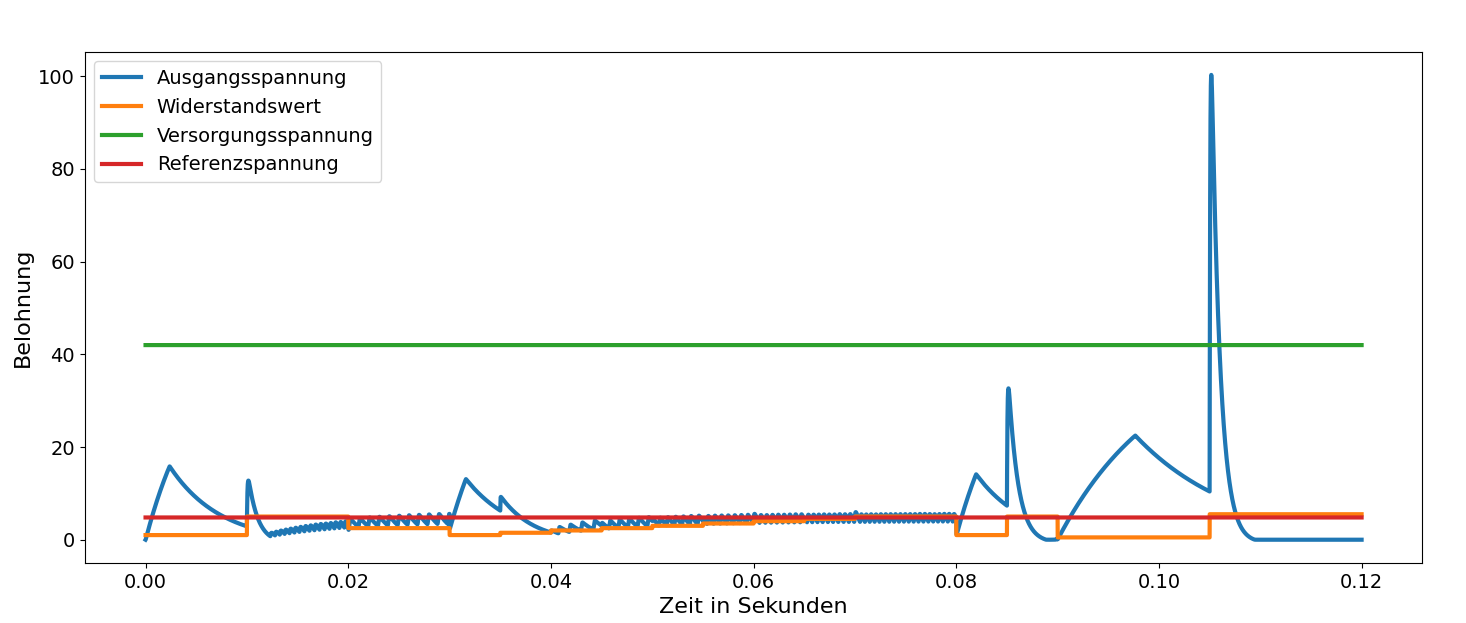
\includegraphics[width=\textwidth]{4Ergebnisse/Phasen/2Phase/TeilIII_2.png}
\caption{Verbesserung der Regelungsleistung des Modells Morpheus während der dritten Phase, illustriert durch die Annäherung der Ausgangsspannung an die Referenzspannung und die Verringerung der Oszillationen.}
\label{fig:phase_iii_morpheus}
\end{figure}

